%%%%%%%%%%%%%%%%%%%%%%%%%%%%%%%%%%%%%%%%%%%
%%% DOCUMENT PREAMBLE %%%
\documentclass[12pt]{article}

\newcommand\attr[2]{%%
  \expandafter\def\csname#1\endcsname{#2}%%
}

\newcommand{\firstpage}{
  \begin{titlepage}
    \centering
      \vspace*{0.5 cm}
    \begin{center}    \textsc{\Large \university}\\[2.0 cm]	\end{center}% University Name
    \textsc{\Large \mastertheme }\\[0.5 cm]				% Course Code
    \rule{\linewidth}{0.2 mm} \\[0.4 cm]
    { \huge \bfseries \thetitle}\\
    \rule{\linewidth}{0.2 mm} \\[1.5 cm]

    \begin{minipage}{0.4\textwidth}
      \begin{flushleft} \large
        \end{flushleft}
        \end{minipage}~
        \begin{minipage}{0.4\textwidth}

        \begin{flushright} \large
          \emph{Student:} \\
          \author \\
          \emph{Professor:} \\
          \professor
      \end{flushright}

    \end{minipage}\\[2 cm]

    \includegraphics[scale = 0.5]{imgs/\universityinitials.png}
  \end{titlepage}
}

\usepackage{agda}
\usepackage{apacite}
\usepackage{catchfilebetweentags}

\usepackage{ucs}
\usepackage{amssymb}

\usepackage[english]{babel}
\usepackage{url}
\usepackage[utf8x]{inputenc}
\usepackage{amsmath}
\usepackage{graphicx}
\graphicspath{{images/}}
\usepackage{parskip}
\usepackage{fancyhdr}
\usepackage{vmargin}
\setmarginsrb{3 cm}{2.5 cm}{3 cm}{2.5 cm}{1 cm}{1.5 cm}{1 cm}{1.5 cm}

\newcommand{\agda}[2]{\ExecuteMetaData[latex/#1.tex]{#2}}
\newcommand{\incimg}[1]{\includegraphics[width=\columnwidth]{imgs/#1}}

\title{Programming a cryptocurrency in Agda}

% Title
\author{Guilherme H. A. Silva}
% Author
\date{15 de Abril de 2019}
% Date

\makeatletter
\let\thetitle\@title
\let\theauthor\@author
\let\thedate\@date
\makeatother

\pagestyle{fancy}
\fancyhf{}
\rhead{\theauthor}
\lhead{\thetitle}
\cfoot{\thepage}
%%%%%%%%%%%%%%%%%%%%%%%%%%%%%%%%%%%%%%%%%%%%
\begin{document}

%%%%%%%%%%%%%%%%%%%%%%%%%%%%%%%%%%%%%%%%%%%%%%%%%%%%%%%%%%%%%%%%%%%%%%%%%%%%%%%%%%%%%%%%%

\firstpage{Fundação Getúlio Vargas}
          {Modelagem Matemática}
          {Guilherme Horta Alvares da Silva}
          {Doctor Flávio Codeço Coelho}
          {FGV}

%%%%%%%%%%%%%%%%%%%%%%%%%%%%%%%%%%%%%%%%%%%%%%%%%%%%%%%%%%%%%%%%%%%%%%%%%%%%%%%%%%%%%%%%%

\tableofcontents
\pagebreak

%%%%%%%%%%%%%%%%%%%%%%%%%%%%%%%%%%%%%%%%%%%%%%%%%%%%%%%%%%%%%%%%%%%%%%%%%%%%%%%%%%%%%%%%%
\renewcommand{\thesection}{\arabic{section}}
\section{Introduction}

\subsection{Context}

In 1983, David Chaum created ecash \cite{panurach1996money} an anonymous cryptographic eletronic money.
This cryptocurrency use RSA blind signatures \cite{chaum1983blind} to spend transactions.
Later, in 1989, David Chaum found an eletronic money corporation called DigiCash Inc.
It was declared bankruptcy in 1998.

Adam Back developed a proof-of-work (PoW) scheme for spam control, Hashcash \cite{back2002hashcash}.
To send an email, the hash of the content of this email plus a nonce has to have a numerically value
smaller than a defined target.
So, to create a valide email, the sender (miner) has to spend a considerable CPU resource on it.
Because, hash functions produces pratically random values, so the miner has to guess a lot of nonce
values before find some nonce that make the hash of the email less than the target value.
This idea is used in Bitcoin proof of work, because each block has a nonce guessed by the miner and
the hash of the block has to be less than the target value.

Wei Dai propose b-money \cite{dai1998b} for the first proposal for distributed digital scarcity.
And Hal Finney created Bit Gold \cite{wallace2011rise}, a reusable proof of work for hashcash for
its algorithm of proof of work.

In 31 October 2008, Satoshi Nakamoto registered the website ``bitcoin.org'' and put a link for his
paper \cite{nakamoto2008bitcoin} in a cryptography mailing list.
In January 2009, Nakamoto released the bitcoin software as open-source code.
The identity of Satoshi Nakamoto is still unknown.
Since that time, the total market of Bitcoin came to 330 billions dollars in 17 of December of 2018
when its value reached the historic peak of 20 thousands dollars.

Other cryptocurrencies like Ethereum \cite{wood2014ethereum}, Monero \cite{noether2015ring} and
ZCash \cite{hopwood2016zcash} were created after Bitcoin,
but Bitcoin is still the cryptocurrency with the biggest market value.

Ethereum is a cryptocurrency that uses account model instead of UTXO used in bitcoin for its
transaction data structure.
It uses Solidity as its programming language for smart contracts which resembles Javascript,
so it is easier to program in it than in the stack machine programming language of Bitcoin.
Ethereum is now transitioning from proof of work (used in Bitcoin) to proof of stake
which will be the default proof mechanism of Ethereum 2.0 and will be released in
3 of January of 2020.

Monero and ZCash are both cryptocurrencies that focus on fungibility, privacy and descentralization.
Monero uses an obfuscated public ledger, so anyone can send transactions,
but nobody can tell the source, amount or destination.
Zcash uses the concept of zero-knowledge proof called zk-SNARKs, which garantee privacy for its users.

\section{Relevant Background}

\subsection{Bibliograph revision}

Before this work, there were some research in this field.
Antom Setzel \cite{setzer2018modelling} already code the definitions of transactions and
transactions tree of bitcoin.
Orestis Melkonian start to formalize Bitcoin Script.

My work try to extend Antom Setzel model and make possible to use Bitcoin protocol
from inputs and outputs from plain text.
For example, the user send a transaction in plain text to the software and it validates if it is correct.
To use the Antom Setzel model, the user has to send the data and the proof that are both valid.

\subsection{Agda Introduction}
Agda is a dependently typed functional language developed by Norell at Chalmers University of Technology
as his PhD Thesis.
The current version of Agda is Agda 2.

  \subsubsection{Syntax}
  In Agda, Set is equal to type.
  In dependent type languages, it is possible to create a function that return a type.

  \agda{agdaExamples}{funcType}

  After the function name, it is two colon (:) and the arguments of the function.
  It is closed by (name\_of\_argument : type\_of\_argument).
  After all, there is one arrow and the type of the result of the function.
  This ``if, then, else'' is not a function built-in in Agda.
  It is a function defined this way if\_then\_else\_ .

  So it is possible to use this function in the default way.

  \agda{agdaExamples}{funcTypeUnd}

  Or use the arguments inside the underscore.

  \agda{agdaExamples}{funcType2}

  The same notation can be done using just arrows without naming the arguments.

  Because of dependent types, it is possible to have a type that depend on the input.

  \agda{agdaExamples}{dependentType}

  It is possible in Agda to do pattern match.
  So it breaks the input in their possible cases.

  \agda{agdaExamples}{patternMatch}

  To create a new type with different pattern match, it is used data constructor.

  \agda{agdaExamples}{dataConstructor}

  This is another example of Data Set, but it depend on the argument.

  \agda{agdaExamples}{vector}

  Vector zero is a type of a vector of size zero, so the only option to construct it is the empty vector.
  It is constructed from the first constructor.
  Other types of vectors like Vector 1 (vector of size one), Vector 2, ... can only be constructed by
  the second constructor.
  It takes as argument a natural number and a vector and return a vector with size of the last vector
  plus one.

  Records are data types with just one case of pattern match.

  \agda{agdaExamples}{record}

  The constructor is the name of data constructor.

  Implicits terms are elements that the compiler is smart enough to deduce it.
  So it is not necessary to put it as argument of the function.

  \agda{agdaExamples}{id}

  Implicits arguments are inside \{\}.
  In this example, the name of the Set (A) can not be omitted
  (like the second function version of boolean to set),
  because it is used to say that x is of type A.

  In case of the function id, the type of the input can be deduced by the compiler.
  For example, the only type that zero can be is Natural.

  \agda{agdaExamples}{idNat}

  Functions in Agda can be defined in two ways

  \agda{agdaExamples}{funcs}

  In the first case, the arguments are before equal sign (=).
  In the second way, it is used the lambda abstraction that mean the same thing.

  \subsubsection{Lambda Calculus}
  Lambda Calculus is a minimalist turing complete programming language with the concept of abstraction,
  application using binding and substitution. For example, x is a variable, $(\lambda x.M)$
  is an Abstraction and (M N) is an Application.

  In Lambda Calculus, there are two types of conversions $\alpha$-conversion and $\beta$-reduction.
  In $\alpha$-conversion, $(\lambda x.M[x]) \rightarrow (\lambda y.M[y])$.
  So in every free variable in M will be renamed from x to y.
  For M[x] = x, an $\alpha$-conversion is $(\lambda x.x) \rightarrow (\lambda y.y)$

  A free variable is every variable that is not bind outside.
  For example, $((\lambda\textcolor{green}{x}.\textcolor{blue}{x}) \textcolor{red}{x})$.
  The \textcolor{blue}{blue x} is binded for the \textcolor{green}{green x},
  but the \textcolor{red}{red x}
  is not binded for any function. So the \textcolor{red}{red x} is a free variable.

  In $\beta$-reduction, it replaces the all free for the expression in the application.
  The $\beta$-reduction of this expression $((\lambda x.M) N) \rightarrow (M[x := N])$ .
  So if $M = x$, the $\beta$-reduction will be $((\lambda x.x) N) \rightarrow N$.
  If $M = (\lambda x.x) x$, the $\beta$-reduction will be
  $(\lambda x.((\lambda x.x)x))N \rightarrow (\lambda x.x)N$.

  Agda uses typed lambda calculus.
  So in an application (M N), M has to be of type $A \Rightarrow B$ and N has to be of type A.
  $(\lambda (x : A) . x)$ is of type $A \Rightarrow A$, because x is of type A.

  \agda{lambdaCalculus}{Id}
  The simplest function is the identity function made in Agda.

  \agda{lambdaCalculus}{Id2}
  This is another way of writing the same function.

  \agda{lambdaCalculus}{trueFalse}
  This is how true and false are encoded in lambda calculus.

  \agda{lambdaCalculus}{naturals}
  This is how naturals numbers are defined in lambda calculus.
  Look that the definition of zero looks like the definition of false.

  \agda{lambdaCalculus}{isZero}
  Defining natural numbers in this way, it is possible to say if a natural number is zero or not.

  \agda{lambdaCalculus}{plus}
  Plus is defined this way using lambda calculus.

  \agda{lambdaCalculus}{onePone}
  This is one example of the calculation of one plus one in Lambda Calculus.

  \agda{lambdaCalculus}{list}
  This is how lists are defined in Lambda Calculus.

  \agda{lambdaCalculus}{sumList}
  Substituting the cons operation of list per plus and nil list to zero, it is possible to calculate
  the sum of the list.

  \agda{lambdaCalculus}{either}
  In this way, it is possible to define Either.
  It is one way to create a type that can be a Natural or a Boolean.

  \agda{lambdaCalculus}{eitherExamples}
  In these examples, it is defined zero, one in left and false, true in right.

  \agda{lambdaCalculus}{eitherRes}
  Either is usefull when defining one function that works for left and another that works for the right.
  The function choosen for left was if a natural number is zero and
  the function choosen for right was if the identity function.

  \agda{lambdaCalculus}{tuple}
  This way is how tuple is defined in Lambda Calculus.

  \agda{lambdaCalculus}{tupleExamples}
  This is how is defined the tuple zero false and the tuple one true.

  \agda{lambdaCalculus}{tupleAdd}
  This is one way of defining a function that add one if the first element of tuple is true.


  \subsubsection{Martin-Löf type theory}
  Agda also provides a proof assistance based on intentional Martin-Löf type theory.

    In Martin-Löf type theory, there are 3 finite types and 5 constructors types.
    The 0 type contain 0 terms, it is called empty type and it is written bot.
    \agda{agdaExamples}{botType}

    The 1 type is the type with just 1 canonical term and it represents existence.
    It is called unit type and it is written top.
    \agda{agdaExamples}{trivialType}

    The 2 type contains 2 canonical terms. It represents a choice between two values.
    \agda{agdaExamples}{eitherType}

    The Boolean Type is defined using the Trivial type and the Either type.
    \agda{agdaExamples}{boolType}

    If statement is defined using booleans.
    \agda{agdaExamples}{ifThenElse}


    \subsubsection{Types Constructors}
    The sum-types contain an ordered pair.
    The second type can depend on the first type.
    It has the same meaning of exist.
    \agda{agdaExamples}{sumType}

    The $\pi$-types contain functions.
    So given an input type, it will return an output type.
    It has the same meaning of a function:
    \agda{agdaExamples}{piType}

    In Inductive types, it is a self-referential type.
    Naturals numbers are examples of that:
    \agda{agdaExamples}{Nat}
    Other data structs like linked list of natural numbers, trees, graphs are inductives types too.

    Proofs in inductive types are made by induction.
    \agda{agdaExamples}{NatElim}

    Universe types are created to allow proofs written in all types.
    For example, the type of Nat is U0.


It looks like CoQ, but does not have tatics.
Agda is a total language, so it is garanteed that the code always terminal and coverage all inputs.
Agda needs it to be a consistent language.

Agda has inductive data types that are similar to algebric data types in non-depently typed programming
language.
The definition of Peano numbers in Agda is:

\agda{agdaExamples}{Nat}

Definitions in Agda are done using induction.
For example, the sum of two numbers in Agda:

\agda{agdaExamples}{sum}

In Agda, because of dependent types, it is possible to make some restrictions in types that is not
possible in other language.
For example, get the first element of a vector.
For it, it is necessary to specify in the type that the vector should have at size greater or equal
than that one.

\agda{agdaExamples}{vecHead}

Another good example is that in sum of two matrices, they should have the same dimentions.

\agda{agdaExamples}{matrixSum}


\subsection{Bitcoin}

The bitcoin was made to be a peer to peer eletronic cash.
It was made in one way that users can save and verify transactions without the need of a trusted party.
Because of that no authority or goverment can block the bitcoin.

\incimg{transactions1.png}

Transactions in bitcoins are an array of input of previous transactions and an array of outputs.
Each input and output is an address, each address is made from public key that is made from a private key.

\incimg{privatekey.png}
%% https://coinsutra.com/bitcoin-private-key/

A private key is a big number.
It is so big that it is almost impossible to generate two identicals private key.

The public key is generated from private key,
but a private key can not be generate from a public key.

The mining transaction does require an input.
For each input of the transaction, it is necessary a signature signed with a private key to prove the
ownership of the bitcoins.
With the message and the signature, it is possible to know that the owner of the private key
that generates the public key signed this message.

With the signature and the public key, it is not possible to know the private key.
So because of that, the owner of the private key can sign several messages without anyone knows
his private key.

\incimg{transactions2.jpg}

Transactions are grouped in a block.
Each block contains in its header the timestamp of its creation, the hash of the block,
the previous hash and a nonce.
A nonce is an arbitrary value that the miner has to choose to make the hash of the block respect some
specific characteristics.

\incimg{blockchain.png}

Each block has a size limit of 1 MB.
Because of that, Bitcoin forms a blockchain (an chain of blocks).
Each block should be created in an average of 10 minutes.
This time was choosen because 10 minutes is enough to propagate the block throughout the world.
To make the blockchain tamper-proof, there is a concept called proof of work in Bitcoin.
So the miner has choose a random value as nonce that makes the hash of the block less
than a certain value.
This value is choosen in a way that each block should be generated in 10 minutes in average.
If the value is too low, miners will take more time to find a nonce that make the hash block
less than the it.
If it is too high, it will be easier to find a nonce and they will find it faster.

When two blocks are mined in nearly the same time, there are two valid blockchains.
It is because the last block in the both blockchains are valid but different.
Because of this problem, in Bitcoin protocol, the largest chain is always the right chain.
While two valid chains have the same size, it is not possible to know which chain is the right.
This situation is called fork and when it happens, it is necessary to wait to see in which chain
the new block will be.

In Bitcoin, there is a possibility of 51\% attack.
It happens when some miner, with more power than all network, mine secretly the blocks.
So if the main network has 50 blocks, the miner could produce hidden blocks from 46 to 55
and he would have 10 hidden blocks from the network.
When he shows their hidden blocks, his chain become the valid chain, because it is bigger.
So all transactions from previous blockchain from 46 to 50 blocks become invalid.
Because of that, when someone make a big transaction in the blockchain, it is a good idea
to wait more time.
So it is becoming harder and harder to make a 51\% with more time.
Bitcoin has the highest market value nowadays, so attacking the bitcoin network is very expensive.
Nowadays, this kind of attack is more common in new altcoins.

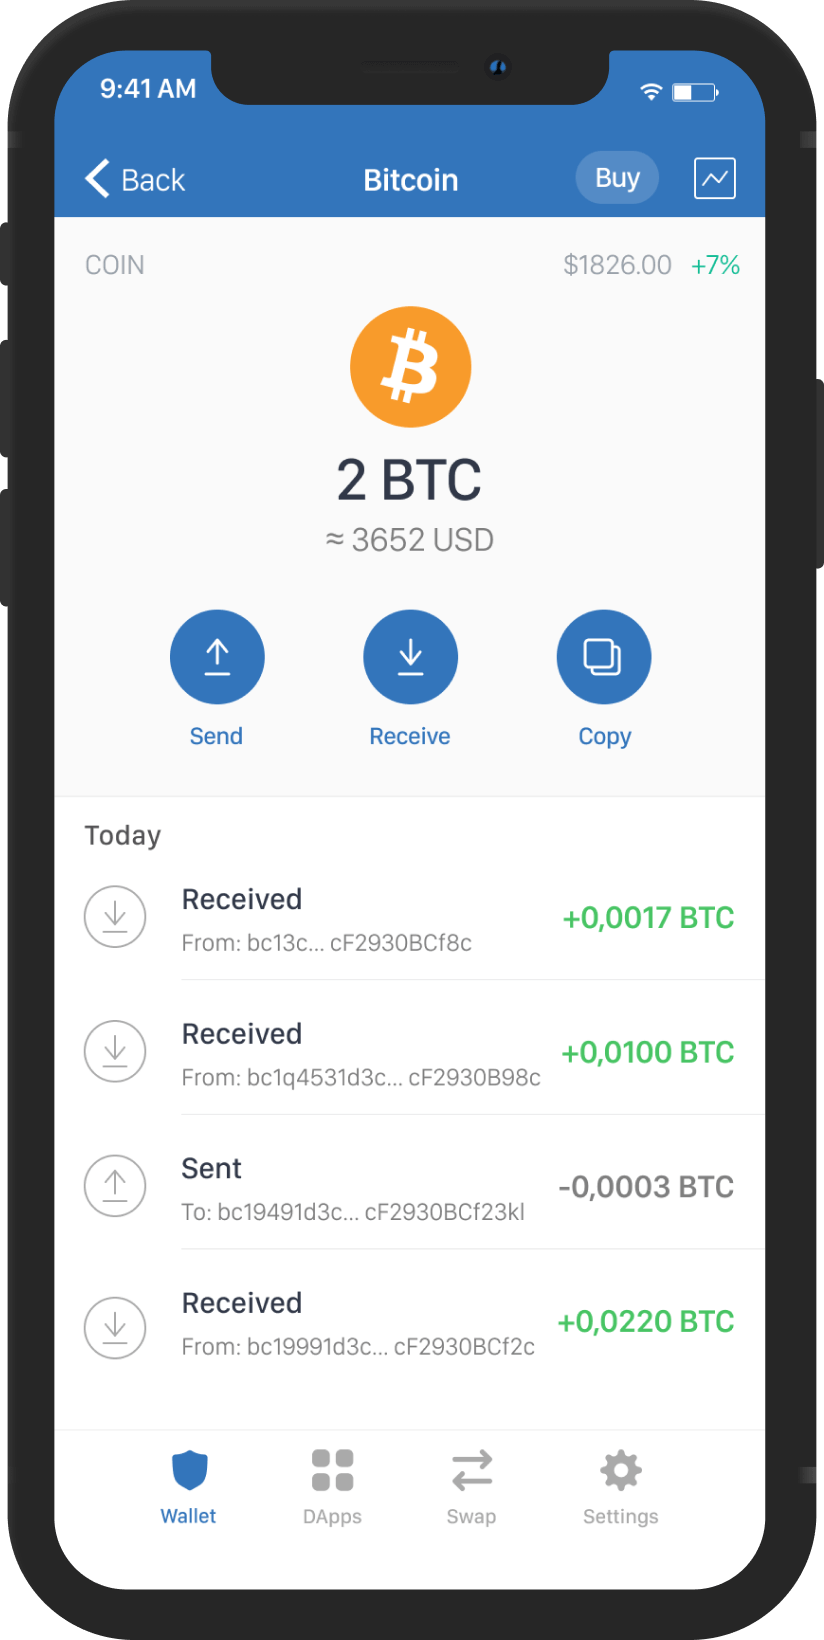
\includegraphics[width=\columnwidth/2]{imgs/wallet.png}
%% https://trustwallet.com/buy-bitcoin/

Wallet is a software that track all transactions that the users received and sent.
It also make new transactions from previous received transactions.

\subsection{Ethereum}

Ethereum differs from bitcoin in having an Ethereum Virtual Machine (EVM) to run script code.
EVM is a stack machine and turing complete while Bitcoin Script is not
(it is impossible to do loops and recursion in Bitcoin).

Transactions in bitcoin are all stored in blockchain.
In Ethereum, just the hash of it is stored in it.
So it is saved in off chain database.
Because of that, it is possible to save more information in Ethereum Blockchain.

In Bitcoin, the creator of the contract as to pay the amount proportional to its size.
In Ethereum, it is different, there is a concept of gas.
Each smart contract in Ethereum is made by a serie of instructions.
Each instruction consume different computional effort.
Because of that, in Ethereum, there is a concept of gas, that measure how much computional effort
each instruction needs.
So in each smart contract, it is well know how much computational effort will be necessary to run it
and it is measured in gas.
Because computional effort is a scarce resource, to execute the smart contract, it is necessary to
pay an amount in Ether for each gas to the miner run it.
Smart contracts that pay more ether per gas run first, because the miner will want to have the best
profit and they will pick them.
If the amount of ether per gas payed is not high enough, the contract will not be executed,
because there are some other contracts that pay more that will be executed instead of this one.

Because Ethereum has its own EVM with more instructions than Bitcoin and it is Turing Complete,
its considered less secure.
Ethereum has its own high level programming language called Solidity that looks like Javascript.

\section{Metodology}

\subsection{Bitcoin UTXO}

There are two kinds of data structures to modeling accounts records and savings states.
The UTXO model used in Bitcoin and the account model used in Ethereum.

  \incimg{account.jpeg}

In account model, it is saved the address and the balance of each address.
For example, the data structure will look like this [(0xabc01, 1.01), (0xabc02, 2.02)].
So the address 0xabc01 has 1.01a of balance and the address 0xabc02 has 2.02 of balance.
In this way, it is possible to easily know how much of balance each address has,
but it is not possible to know how they got in this state.

  \incimg{utxo.png}

In UTXO model, each transaction is saved in the transaction tree.
Every transaction is composed of multiples inputs and multiples outputs.
But all inputs have to never been spent before.

Because of that, in UTXO model, it is easy to make a new transaction from previous one, but it is harder
to know how much each one has.
The wallet that calculate how much balance each address has.

In account model, there could be one kind of vulnerability that is less probabable to happen in UTXO
model.
Because there is an undesirable intermediary state that there is some address without balance while
another has not already received his money.

For example: \\
bobBalance -= 1 \\
Intermediary State \\
aliceBalance += 1

In account model, it is straight foward to know how much balance each address has.
In UTXO model, this calculation is made offchain. It can be a good thing,
because each user has more privacy.

\subsection{Cripto Functions}
The first thing that we define are the cripto functions that will be needed to make the criptocurrency.
Messages can be defined in multiple ways, one array of bytes, one string or a natural number.
Messages in this context means some data.

Private key is a number, a secret that someone has.
In Bitcoin, the private key is a 256-bit number.
Private key is used to signed messages.

Public key is generated from private key.
But getting private key from public key is impossible.
To verify who signed a message with a private key, he has to show the public key.

Hash is an injection function (the probability of collision is very low).
The function is used from a big domain to a small domain.
For example, a hash of big file (some GBs) is an integer of just some bytes.
It is very usefull to prove for example that 2 files are equal.
If the hash of two files are equal, so the files are equal.
It is used in torrents clients, so it is safe to download a program to untrusted peers,
just have to verify if the hash of the file is equal to the hash of the file wanted.

These functions can be defined, but it is not the purpose of this theses.
So they will be just postulates.

\agda{Cripto}{criptoPostulates}

\subsection{Transactions}

In Bitcoin, there are some transactions.
In each transactions, there are multiple inputs and outputs.
Each input is named TXFieldWithId.
The input of one transaction is the ouput of another transaction.
Firsts outputs are generated from coinbase transaction (there is just one of this transaction at
each block).
Coinbase transactions are the miner reward.

\agda{Transactions}{VectorOutput}

Vector output is the vector of outputs transactions.
It is a non empty vector.
In its representation, it is possible to know in what time it was created (time is the position of
they in all transactions),
what is his size (quantity of outputs fields)
and the total amount spend in this transaction,

elStart is a proof that the position of TXFieldWithId is the last one.
It is used after to specify wich input is in the transaction.

\agda{Transactions}{TXSigned}

A signed transaction is composed of a non empty list of inputs and outputs.
For each input, there is a signature that confirms that he accepted every output in the list of outputs.
And in the transaction, there is a proof that the total amount of money in all inputs are bigger than
the total amount of outputs.
The remainder will be used by the miner.

\subsection{Transaction Tree}

Transaction tree is one of most important data structures in bitcoin.
In the transaction tree, there are all unspent transaction outputs (UTXO).
In every new transaction, the UTXOs used as input is removed from transaction tree.

\agda{TXTree}{TXTree}

In this implementation, time is the number of the transactions in TXTree.
Block is related in which block the transaction tree is.
After every new coinbase transaction (the miner transaction), the block size increment in one quantity.
Total fees are how much the miner will have in fee of transactions if he makes a block with these
transactions.
Quantity of transactions is how many transactions there are in the current block.
The type is tQtTxs instead of a natural number, because in this implementation, each block can has
a number maximum of transactions.
In bitcoin, it is different, each block has a limit size in space of 1 MB.

Genesis tree is the first case.
It is when the crypto currency was created.
txtree is created from another tree.
proofLessQtTX is a proof that the last transaction tree has its
block size less than the maximum block size minus one or it is a coinbase transaction.
It is because, it is necessary to verify the size of the last txtree so it will not have
the size greater than the maximum.

\agda{TXTree}{TX}

TX is related to the transaction done in the cripto currency.
There are two kinds of transaction.
Coinbase transaction is the transaction done by the miner.
In coinbase, they have just outputs and do not have any input.
pAmountFee is a proof that the output of coinbase transaction is equal to the total fees plus
a block reward.

Another kind of transaction is the normalTX, a regular transaction.
SubInputs are a sub list of all unspent transaction outputs of the previous transaction tree.
Outputs are the new unspent transaction from this transaction.
So who receive the amount from this transaction can spend it after.
TxSigned is the signature that proves that every owner of each input approve this transaction.
In TxSigned, there is a proof that the output amount is greather than the input amount too.

\agda{TXTree}{isCoinBase}

This function just return trivial type if coinbase and bot type if not.

\agda{TXTree}{nextBlock}

If it is a normal transaction, the block continue the same.
If it is a coinbase transaction, the next transaction will be in a new block.

\agda{TXTree}{incQtTx}

This function is to increment the quantity of transaction in the block.
It has to receive a proof that the quantity of transaction that was before this new transaction was
less than then maximum quantity of transaction allowed.
So it is guaranteed that the quantity of transactions will never be greater than the maximum allowed.
If it is a coinbase transaction, it will be a new block.
So the quantity of transactions start being zero.

\agda{TXTree}{incFees}

IncFee is a function that increment how much fee the miner will receive.
If it is a coinbase transaction, the fee will be received by the miner,
so the next miner will not receive this previous fee.
Because of that, the new fee will start from zero.
If it is a normal transaction, the newest fee will be the amount of input of the transaction minus
the output of this trasaction plus the last fee of previous transactions.

\agda{TXTree}{outFee}

outFee+RewardBlock is a proof that the amount of output transactions is equal to total fees of
others transactions plus the block reward.

\subsection{Blockchain}

Block is a chain of transaction that is added in Bitcoin blockchain in every ten minutes.
Each block consisit of serveral transactions and a miner transaction.
This is how block in defined in this work:

\agda{Blockchain}{block}

nextTXTree assure that the second transaction tree is from the first transaction tree.
firstTreesInBlock garantee that the last transaction in the first transaction tree
is the first in the block.
coinBaseTree assure that the last  transaction in the second transaction tree is
a coinbase transaction.

Blockchain is a chain of valid blocks.
Every new block must be a continuation of the previous one.
Here is the definition of the blockchain:

\agda{Blockchain}{blockchain}

In the first case, blockchain just has one block, called fstBlock.
In the second case, the blockchain is an addition of a valid block from a previous blockchain.

\section{Conclusion}

\newpage

\bibliographystyle{apacite}
\bibliography{References}

\end{document}
